\documentclass[12pt]{article}
\usepackage{standalone}
\usepackage[italian]{babel}
\usepackage[margin=2cm]{geometry}
\usepackage{graphicx}
\usepackage{hyperref}

\usepackage{enumitem} %this is needed to resume an itemization (https://stackoverflow.com/questions/1348194/how-to-interrupt-resume-a-list-in-latex) 


\renewcommand{\familydefault}{\sfdefault}
\usepackage{mathpazo,hyperref}
\usepackage{amsthm,amsmath,amssymb}
%\newcommand\soluzione[1]{\footnote{#1}}
\newcommand\soluzione[1]{}



\setlength{\parindent}{0 em}
\setlength{\parskip}{1 em}

\author{}
\title{Indicazioni per lo svolgimento delle esercitazioni}



\begin{document}
\maketitle
\tableofcontents

\vfill\newpage
\section{Regolamento per le esercitazioni}
\begin{itemize}
\item Le esercitazioni vengono proposte tramite la piattaforma moodle e costituiscono parte integrante dell'esame.

  \item Le esercitazioni devono essere caricate sulla piattaforma moodle entro il giorno precedente all'appello.

\item  In fondo ad ogni elaborato dovrete scrivere una breve dichiarazione firmata che attesti che l'elaborato \`e frutto del vostro lavoro.

  \end{itemize}


\section{Modalit\`a di consegna}
\begin{itemize}
\item  Le esercitazioni vanno scritte a mano, preferibilmente su carta bianca (ma anche su foglio a quadretti o righe, purch\'e la scansione sia leggibile), scansionate  e convertite in formato \texttt{PDF} o \texttt{JPG} adoperando una delle tante app gratuite disponibili (ad esempio \texttt{camscanner}, in modo che lo sfondo sia bianco e non opaco.
  
\item Nella versione pi\`u recente, il sistema moodle  impone il limite di 20MB alla dimensione di ciascun file caricabile. Qualora le dimensioni del file ottenuto con il programma di scansione risultassero superiori a questo limite, sar\`a sufficiente suddividere il compito tra pi\`u file.

  \item Avvertenza: se si tenta di caricare un file di dimensioni maggiori di 20MB, il sistema non salva il file e non segnala l'errore, illudendo l'utente che il caricamente sia andato a buon fine. {\bf Si consiglia di verificare sempre che il compito sia stato caricato correttamente}. Poich\'e il limite alla dimensioni dei file da caricare sulla piattaforma elettronica \texttt{moodle} \`e relativamente basso, si consiglia di fare qualche prova per evitare di trovarsi nella spiacevole situazione di non poter caricare gli svolgimenti dei compiti nei tempi stabiliti.

  \item In caso di segnalazioni relative a questioni sui compiti, il sistema permette di aggiungere commenti durante il caricamente del compito.

\item NOTA: Non si devono allegare le foto dei compiti (queste risultano difficilmente leggibili sullo schermo e illegibili se stampate) al posto delle scansioni.

  \end{itemize}


  
\section{Indicazioni per la redazione  delle esercitazioni}

Le esercitazioni devono essere redatte come se si trattasse dell'esposizione della risoluzione di un problema su un libro di testo. 

\paragraph{Indicatori.} Gli indicatori che verranno adoperati per la valutazione delle esercitazioni sono i seguenti:
\begin{itemize}
\item Completezza dell'esposizione: capacit\`a di includere nel testo tutti gli elementi necessari alla comprensione del discorso;
\item Sintesi, cio\`e capacit\`a di evitare di includere nel testo elementi non necessari alla comprensione;
\item Rigore espositivo, inteso come capacit\`a di concatenare le argomentazioni in modo che siano ciascuna una conseguenza logica dell'altra;
\item Rispetto delle regole della grammatica;
\item Rispetto delle regole della costruzione del periodo;
\item Utilizzo corretto del vocabolario;
\item Correttezza dimensionale dei calcoli;
\item Correttezza numerica dei calcoli.
\end{itemize} 
Si consiglia, prima di consegnare il compito, di far leggere il testo ad un collega affinch\'e  esprima un voto su ciascuno dei punti sopra elencati. Si ribadisce che questi indicatori saranno adoperati in sede di valutazione delle prove scritte. \`E quindi importante tenerli presenti durante la redazione dei compiti a casa.


\paragraph{Struttura del testo.}
Anche se contiene formule e figure, lo svolgimento di un problema deve essere un testo strutturato secondo le regole della grammatica e della sintassi della lingua italiana. In particolare, 
\begin{enumerate}
  \item \label{punteggiatura} Vanno rispettate le regole della punteggiatura.
\item {\bf Ogni singola parola} che presente nel compito deve far parte di una {\bf proposizione}, ovvero, di frase di senso compiuto.
\item Ogni proposizione deve far parte di un periodo, essere correttamente collocata in un contesto sintattico (essere collegata con le altre frasi da opportune congiunzioni.
\item  {\bf Le formule matematiche vanno trattate come frasi}. Come tali, devono essere collegate con il resto del periodo da opportuni costrutti. Ci\`o vale anche se la formula \`e collocata ``in mostra'', come spiegato pi\`u avanti;
\item Le regole della punteggiatura valgono anche se un periodo contiene delle formule (in particolare, ogni periodo che termini con una formula deve essere delimitato da un punto).
\item Il flusso degli argomenti e delle formule deve essere lo stesso di un tema: dall'inizio della pagina fino in fondo; evitare di fare riferimento a formule che appaiono sotto, a destra o a sinistra.
\end{enumerate}

Inoltre, lo svolgimento deve seguire gli elementari dettami del rigore espositivo:\
\begin{enumerate}[resume]
\item \label{pippo} i simboli devono essere essere definiti prima di essere adoperati;
\item ogni passaggio deve essere argomentato e giustificato, richiamando sinteticamente le eventuali nozioni pregresse necessarie alla sua interpretazione, citando una fonte bibliografica (a meno che non si tratti di nozioni elementari insegnate nei corsi di base) oppure facendo riferimento alle lezioni.
\end{enumerate}

\paragraph{Utilizzo delle formule ``in mostra''.} Per quanto riguarda il posizionamento delle formule nel testo occorre fare la seguente precisazione: nelle regole redazionali di uso corrente \`e ammesso che una formula matematica, pur facendo parte di una frase, costituisca l'unico elemento di una riga, eventualmente accompagnata da una numerazione all'estremo di destra della riga in questione. Si dice che tale formula appare ``in mostra''. 

Le formule in mostra sono un accorgimento tipografico utile --- se non indispensabile --- qualora sia necessario riferirsi ad una formula in punti successivi del testo. Tale accorgimento viene adoperato per mettere in evidenza i passaggi fondamentali di una certa argomentazione. Non esiste una regola per stabilire se una formula appaia in mostra oppure no. Troppe formule tra le righe rendono difficoltoso seguire una argomentazione matematica. Troppe formule in mostra richiano di disorientare il lettore. 

Sta all'abilit\`a di chi scrive scegliere la combinazione migliore di formule in mosttra e formule tra le righe. Di norma, bisogna decidere in anticipo quali sono le formule sulle quali vogliamo che cada l'occhio del lettore e nascondere tra le righe le formule che, pur essendo necessarie per comprendere i passaggi tra due formule esibite in mostra, non veicolano concetti importanti.


\vfill\newpage
\section{Griglia di valutazione degli elaborati}
Gli elaborati previsti nel corso e nell'esame sono essenzialemnte di due tipi: svolgimento di un problema che preveda una risposta quantitativa (ad esempio, un problema o un esercizio); svolgimento di un tema o risposta ad un quesito che preveda una risposta di tipo qualitativo (ad esempio, una domanda o un problema sulla teoria). Nel secondo caso, le aree di valutazione sono solo le prime tre e i pesi vanno rinormalizzati in modo che la loro somma dia 100 (ossia, vanno moltiplicati per 100/45).
\begin{table}[h]
  \centering
  \begin{tabular}[l]{|l|l|c|}
\hline
Area & Indicatori & Peso \\ 
\hline
Chiarezza espositiva                           
& \parbox{20em}
{\quad
\\ Intellegibilit\`a e pulizia della grafia. 
\\ Formattazione del testo.
\\  Organizzazione della esposizione.
\\ Consequenzialit\`a delle argomentazioni. \\
} & 20\% \\
\hline
Propriet\`a di linguaggio                      
& 
\parbox{20em}{\quad\\
Aderenza alle regole della grammatica e della sintassi.
\\ Uso corretto del vocabolario. 
\\ Padronanza della terminologia tecnica.\\}                               & 15\% \\
\hline
    Capacit\`a di sintesi                         
& 
\parbox{20em}{\quad\\Capacit\`a di sfruttare lo spazio consentito.
\\Capacit\`a di selezionare le argomentazioni pertinenti alla traccia.\\ 
Capacit\`a di selezionare i dettagli rilevanti.\\} & 15\% \\
\hline
Correttezza qualitativa & \parbox{20em}{\quad\\Correttezza dei procedimenti adoperati per giungere ad un dato risultato. \\ Capacit\`a di dare risposte adoperando considerazioni di carattere qualitativo. \\Padronanza delle dimensioni fisiche \\ Utilizzo corretto delle cifre significative.} & 15\% \\
\hline
Correttezza quantitativa                           & \parbox{20em}{\quad\\Capacit\`a di approssimare l'ordine di grandezza \\ Capacit\`a di approssimare il valore\\} & 25\% \\
\hline
  \end{tabular}
  \caption{Elementi adoperati per la valutazione di un elaborato}
  \label{tab:valutazione}
\end{table}


%\end{document}
\vfill\newpage
\section{Un esempio.}
Si riporta un esempio di analisi di un compito svolto a casa. 

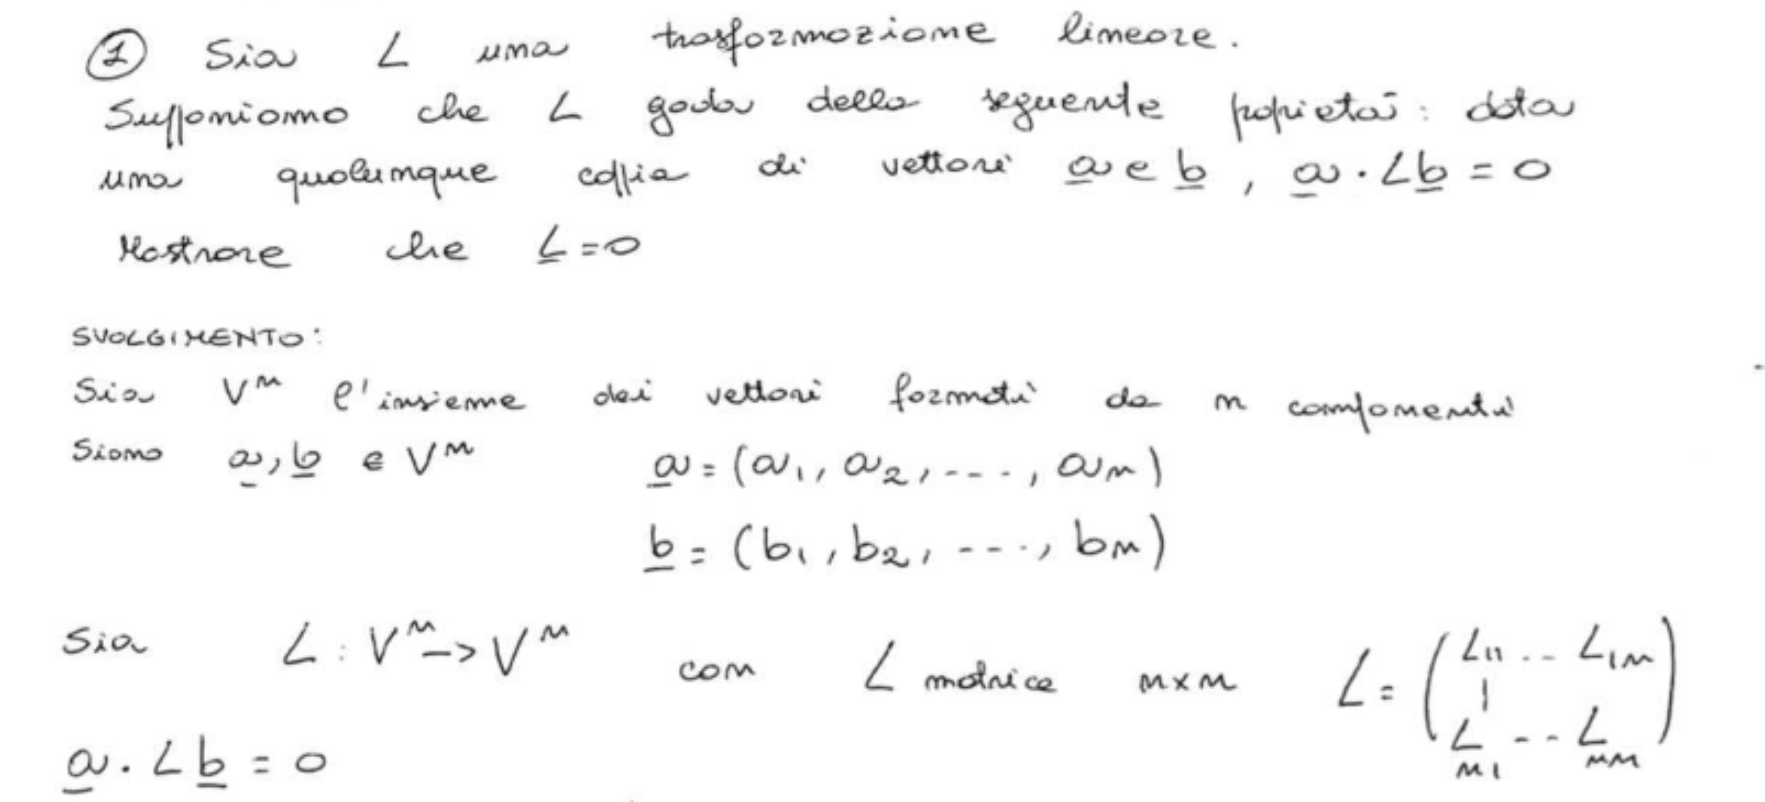
\includegraphics[width=\linewidth]{capture.png}

%Pensare che i compiti assegnati per casa siano delle ``esercitazioni'' tradisce la seguente nozione errata di cosa sia lo studio universitario: la materie studiate in un corso universitario non sono un insieme di nozioni da apprendere e sulle quali fare esercizi.

Per quanto riguarda la forma, osserviamo che:
\begin{itemize}
  \item La calligrafia \`e buona e intellegibile. Emerge in maniera molto chiara la cura dell'autore per la grafia. Le parole sono ben distanziate e i margini sono ben definiti. 
\item  
  Nel terzo periodo manca una virgola dopo $L:V^n\to V^n$  e un articolo indeterminativo prima della parola ``matrice''. Inoltre, la formula $L=\begin{pmatrix}L_{11}\ldots L_{1n}\\L_{n1}\ldots L_{nn}\end{pmatrix}$, che \`e una frase, non costituisce un periodo, poich\'e non circoscritta dalla punteggiatura, n\'e fa parte di un periodo pi\'u ampio, poich\'e non \`e collegata alle altre frasi tramite una qualche congiunzione; tale frase si pone dunque al di fuori del contesto sintattico.
  
\item Per quanto riguarda l'impaginazione, si rileva che alcune frasi (nella fattispecie, le formule $\mathbf a=(a_1,\ldots, a_n)$) sono collocate in modo da rendere equivoca la loro appartenenza ad un eventuale periodo.  

\item Si rileva la mancanza dei punti di chiusura alla fine del  periodo (Indicazione \ref{punteggiatura}). Essendo questo errore ripetuto sistematicamente, il docente non lo interpreta come una svista.
\end{itemize}

Osservazioni sul contenuto.
\begin{itemize}
\item Dal terzo periodo traspare un errore concettuale: l'autore confonde una matrice, ovvero una tabella di scalari, con una generica applicazione da $V^n$ a $V^n$, senza peraltro indicare che la applicazione in questione \`e lineare (senza questa ipotesi non possiamo pensare a $\mathbf L$ come a una matrice). Sarebbe stato corretto dire che $L:V^n\to V^n$ \`e una trasformazione lineare e che la matrice $\mathbf L$ ne costituisce la rappresentazione in una base.

\item Il fatto che nel terzo periodo l'autore abbia ripetuto parte dell'enunciato posto all'inizio della pagina manifesta l'intenzione di riproporre nello svolgimento i dettagli dell'enunciato stesso. Il lettore si aspetta dunque che i periodi con cui inizia lo svolgimento del compito rappresentino una riscrittura delle ipotesi dell'enunciato che si vuole dimostrare.

  In questo contesto, la frase sintetizzata nella formula $\mathbf a\cdot\mathbf L\mathbf b=0$, posta in fondo, ha un significato equivoco: non essendo inserita in un contesto sintattico come frase subordinata, essa {\bf rappresenta una affermazione da interpretarsi come ipotesi su $\mathbf a$, $\mathbf b$, e $\mathbf L$}, a fronte di una ipotesi che riguarda solamente $\mathbf L$. L'autore ci sta dicendo che ha scelto $\mathbf a$ e $\mathbf b$ in modo che $\mathbf a\cdot\mathbf L\mathbf b=0$. 
\end{itemize}


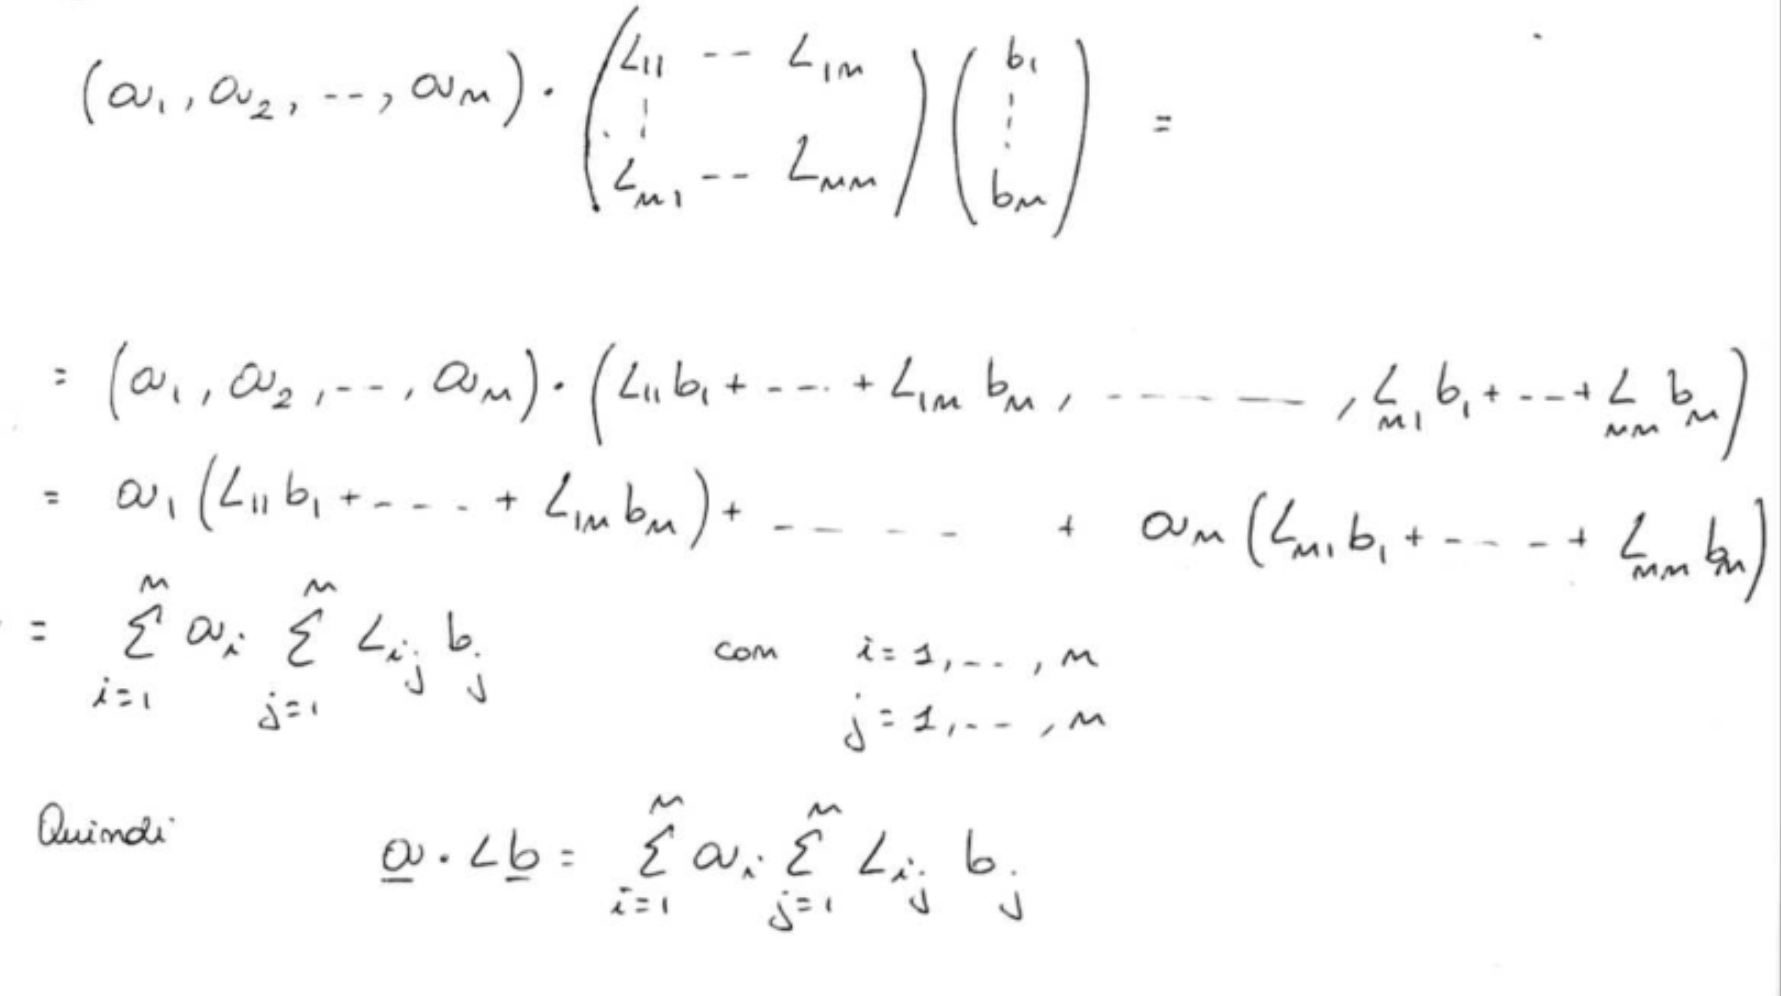
\includegraphics[width=\linewidth]{capture2.png}

Osservazioni sulla forma:
\begin{itemize}
\item Inserire il punto tra il vettore riga $\mathbf a^T=(a_1,\ldots,a_n)$ e il vettore colonna ottenuto moltiplicando la matrice $\mathbf L$ per il vettore $\mathbf b$ \`e concettualmente sbagliato, dato che  il prodotto scalare tra vettori riga e vettori colonna non \`e definito. Risulta definito il prodotto riga per colonna tra il vettore riga $\mathbf a^T$ e il vettore colonna $\mathbf L\mathbf b$:
\begin{equation}
  \mathbf a^T\mathbf L\mathbf b.
\end{equation}
Risulta anche definito il prodotto
\begin{equation}
  \mathbf a\cdot\mathbf L\mathbf b.
\end{equation}
Non risulta per\`o definito il prodotto $\mathbf a^T\cdot\mathbf L\mathbf b$.

\item Specificare, in fondo alla prima formula, che gli indici $i$ e $j$ variano tra $1$ e $n$ \`e sia superfluo che dannoso. \`E superfluo perch\'e l'intervallo di variazione di questi indici \`e sottinteso nel loro impiego sotto i simboli di sommatoria. \`E dannoso perch\'e il lettore, vedendo la specifica di un intervallo per l'indice $i$ in fondo alla formula si aspetta che quell'indice siano liberi, anzich\'e muti, e che la formula sia vera solo se i valori di quei indici cadono in un determinato intervallo.

\end{itemize}


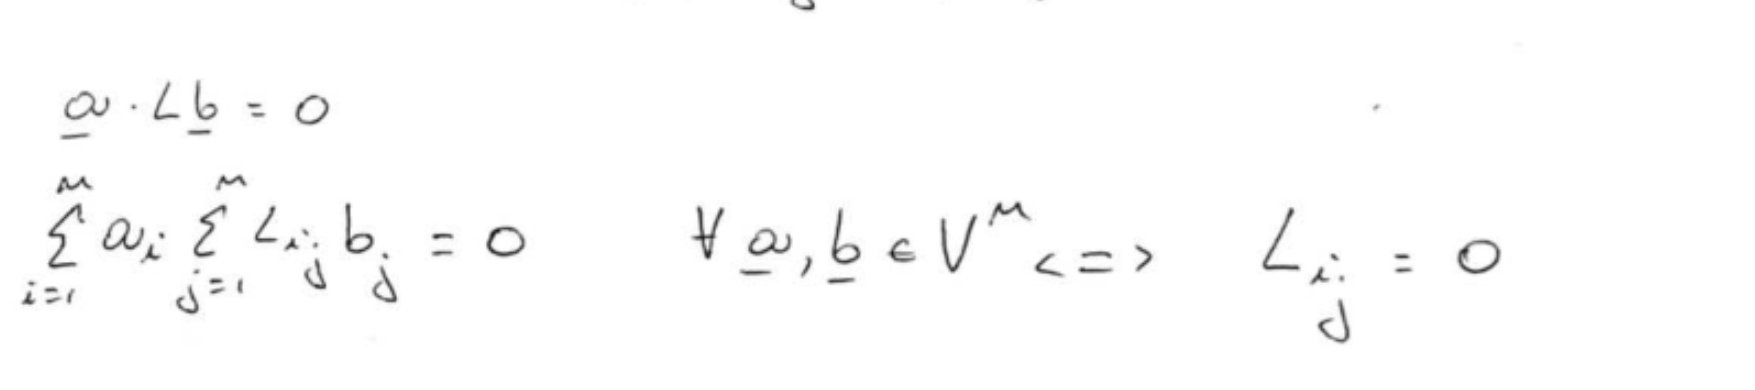
\includegraphics[width=\linewidth]{capture3.png}


Osservazioni sulla forma:
\begin{itemize}
\item Ancora una volta, non si capisce il nesso sintattico tra le frasi contenute in questo frammento di compito. Come sono scelti i vettori $\mathbf a$ e $\mathbf b$? Sono vettori arbitrari?
\end{itemize}

Osservazioni sul contenuto:

\begin{itemize}
 \item Quello che probabilmente l'autore intende essere l'ultimo periodo del compito, non \`e altro che una riscrittura dell'enunciato da dimostrare. Dunque il compito \`e da intendersi non svolto.
 \end{itemize}

 Valutazione sintetica:

 Chiarezza espositiva: insufficiente.

 Propriet\`a di linguaggio: insufficiente.

 Capacit\`a di sintesi: sufficiente.

 Correttezza qualitativa: insufficiente.

 Correttezza quantitativa: non valutata.

 Valutazione complessiva: insufficiente.
\end{document}